% =====================================================================
%  The Shape of the Threat — preamble
%  Identity, type system and page furniture.
%  Every field here is fixed by the owner except \bookDOI, which is
%  per-book and lives in exactly one place so it can be swapped in
%  a single edit.
%
%  Typeset with XeLaTeX.
% =====================================================================

% ---- Standing book identity -------------------------------------------
\newcommand{\bookTitle}{The Shape of the Threat}
\newcommand{\bookSubtitle}{Characterising Near-Earth Objects for Impact Accountability, and the Case for a Lunar Surface Array}
\newcommand{\bookAuthor}{Gerald Enrique Nelson Mc Kenzie}
\newcommand{\bookImprint}{Tico Internet LLC}
\newcommand{\bookEdition}{2026 First Edition}
\newcommand{\bookLicense}{Apache License 2.0}
\newcommand{\bookDOI}{10.5281/zenodo.24517244}   % <-- the one field that changes
\newcommand{\bookFactsDate}{24 November 2026, 22:00 UTC}
\newcommand{\bookCopyright}{2026}

% =====================================================================
%  Colour engine — loaded first, the tokens below need it
% =====================================================================
\usepackage[table]{xcolor}

% =====================================================================
%  DESIGN TOKENS
%  One palette, one type system. Change a value here and the whole
%  book follows.
% =====================================================================
% Palette — an observatory at night: indigo ground, sodium-gold accent,
% a cooler blue reserved for caveats and counter-evidence.
\definecolor{dbg}{HTML}{080B14}        % page background
\definecolor{panel}{HTML}{121828}      % card / table tint
\definecolor{paneledge}{HTML}{27324C}  % card border, hairlines
\definecolor{accent}{HTML}{E8B85C}     % the single accent
\definecolor{accentdim}{HTML}{8A7238}  % accent at low emphasis
\definecolor{txt}{HTML}{E6E9F0}        % body text
\definecolor{txtdim}{HTML}{939BAB}     % secondary text, captions, folios
\definecolor{gridline}{HTML}{141A28}   % background grid
\definecolor{amber}{HTML}{6FA3D6}      % used only for caveats

% Type scale (points) — sizes follow the design system, not habit
\newcommand{\szDisplay}{30}    % cover title
\newcommand{\szTitle}{17}        % part / chapter title
\newcommand{\szSection}{12.4}      % section
\newcommand{\szSub}{10.6}      % subsection
\newcommand{\szBody}{10.2}     % body
\newcommand{\szCaption}{8.2}   % captions
\newcommand{\szMeta}{7.4}     % running heads, folios

% ---- Package stack ------------------------------------------------------
\usepackage{fontspec}
\usepackage{unicode-math}
\setmainfont{Outfit}[
  UprightFont={Outfit Regular}, BoldFont={Outfit Bold},
  ItalicFont={Outfit Regular}, ItalicFeatures={FakeSlant=0.20},
  BoldItalicFont={Outfit Bold}, BoldItalicFeatures={FakeSlant=0.20},
  Ligatures={TeX}]
\setsansfont{Outfit}[
  UprightFont={Outfit Regular}, BoldFont={Outfit Bold},
  ItalicFont={Outfit Regular}, ItalicFeatures={FakeSlant=0.20},
  BoldItalicFont={Outfit Bold}, BoldItalicFeatures={FakeSlant=0.20},
  Ligatures={TeX}]
\setmonofont{DejaVu Sans Mono}[
  UprightFont={DejaVu Sans Mono}, BoldFont={DejaVu Sans Mono Bold},
  ItalicFont={DejaVu Sans Mono}, BoldItalicFont={DejaVu Sans Mono Bold},
  ItalicFeatures={FakeSlant=0.20}, Ligatures={TeX}]
% Fira Math ships a single weight in this TeX Live installation. The book
% uses no bold mathematics, so bold maps to the regular face; if bold maths
% is ever added, install FiraMath-Bold and point BoldFont at it.
\setmathfont{FiraMath-Regular.otf}[
  Path=/usr/share/texlive/texmf-dist/fonts/opentype/public/firamath/,
  Extension = .otf, Ligatures = {TeX}, Scale = 1.0,
  BoldFont = FiraMath-Regular.otf]

\usepackage{textcomp}
\usepackage{amsmath,bm}
\usepackage{ragged2e}
\usepackage{fvextra}
\fvset{
  breaklines=true,
  breakanywhere=true,
  breaksymbolleft={},
  breaksymbolright={},
  fontsize=\footnotesize,
  baselinestretch=1.0
}
\RecustomVerbatimEnvironment{verbatim}{Verbatim}{
  breaklines=true,
  breakanywhere=true,
  breaksymbolleft={},
  breaksymbolright={},
  fontsize=\footnotesize
}
% XeTeX performs character protrusion itself, from the font's own tables.
% microtype's protrusion tables are meant for pdfTeX, and its inheritance
% list for the TU encoding asks for slots that a Unicode encoding does not
% provide, so it warns twice about characters it never sets here. Turning
% microtype's own protrusion off leaves the engine's protrusion in place and
% the warning out of the log; the typesetting is byte for byte the same.
\usepackage[protrusion=false]{microtype}
\usepackage{graphicx}
\usepackage{tikz}
\usepackage{pgfplots}
\usepackage{booktabs}
\usepackage{tabularx}
\usepackage{longtable}
\usepackage{array}
% ---- Table columns -------------------------------------------------------
% Prose inside a table is set ragged right.  A justified column at this
% measure stretches the inter-word space to fill the line, and a narrow
% justified column breaks words; both are worse in a table than a loose
% line.  P is a fixed-width prose column and Y is the column that takes
% the remaining width.
\newcolumntype{P}[1]{>{\RaggedRight\arraybackslash}p{#1}}
\newcolumntype{Y}{>{\RaggedRight\arraybackslash}X}
\usepackage{multirow}
\usepackage{makecell}
\usepackage{enumitem}
\usepackage{float}
\usepackage{caption}
\usepackage{tcolorbox}
\tcbuselibrary{skins,breakable}
\usepackage{fancyhdr}
\usepackage{titlesec}
\usepackage{tocloft}
\usepackage{pdfpages}
\usepackage{eso-pic}
\usepackage{url}
\urlstyle{tt}
\usepackage{seqsplit}
% Long identifiers and DOIs are quoted from the literature and are far
% wider than a 4.6 in measure; \code breaks them between characters.
\newcommand{\code}[1]{\texttt{\seqsplit{#1}}}
\usepackage[bookmarksdepth=3]{hyperref}
\usepackage{makeidx}
\usepackage{etoolbox}
\usepackage[english]{babel}

\pgfplotsset{compat=1.18}

% ---- Page geometry: 6 x 9 in trim --------------------------------------
\usepackage[
  paperwidth=6in, paperheight=9in,
  inner=0.80in, outer=0.60in,
  top=0.82in, bottom=0.78in,
  headheight=14pt, headsep=16pt,
  footskip=28pt
]{geometry}

% ---- Page colour -------------------------------------------------------
\pagecolor{dbg}
\color{txt}

% ---- Paragraph and list rhythm -----------------------------------------
\setlength{\parindent}{0pt}
\setlength{\parskip}{5.5pt plus 1pt}
\linespread{1.06}
\raggedbottom
\widowpenalty=10000
\clubpenalty=10000
\sloppy

\setlist[itemize]{leftmargin=1.15em,itemsep=3.5pt,topsep=4pt,parsep=0pt,
  label=\textcolor{accent}{\textbullet}}
\setlist[enumerate]{leftmargin=2.9em,itemsep=3.5pt,topsep=4pt,parsep=0pt,
  label=\textcolor{accent}{\ttfamily\theenumi.}}
\renewcommand{\labelitemii}{\textcolor{accent}{\textendash}}

% ---- Background grid for openers ---------------------------------------
% The grid motif appears on part and chapter openers only: it reads as
% design there, and as noise behind body text. Coordinates are in inches,
% measured from the lower-left corner of the page.
\newcommand{\gridlayer}{%
  \AddToShipoutPictureBG*{%
    \AtPageLowerLeft{%
      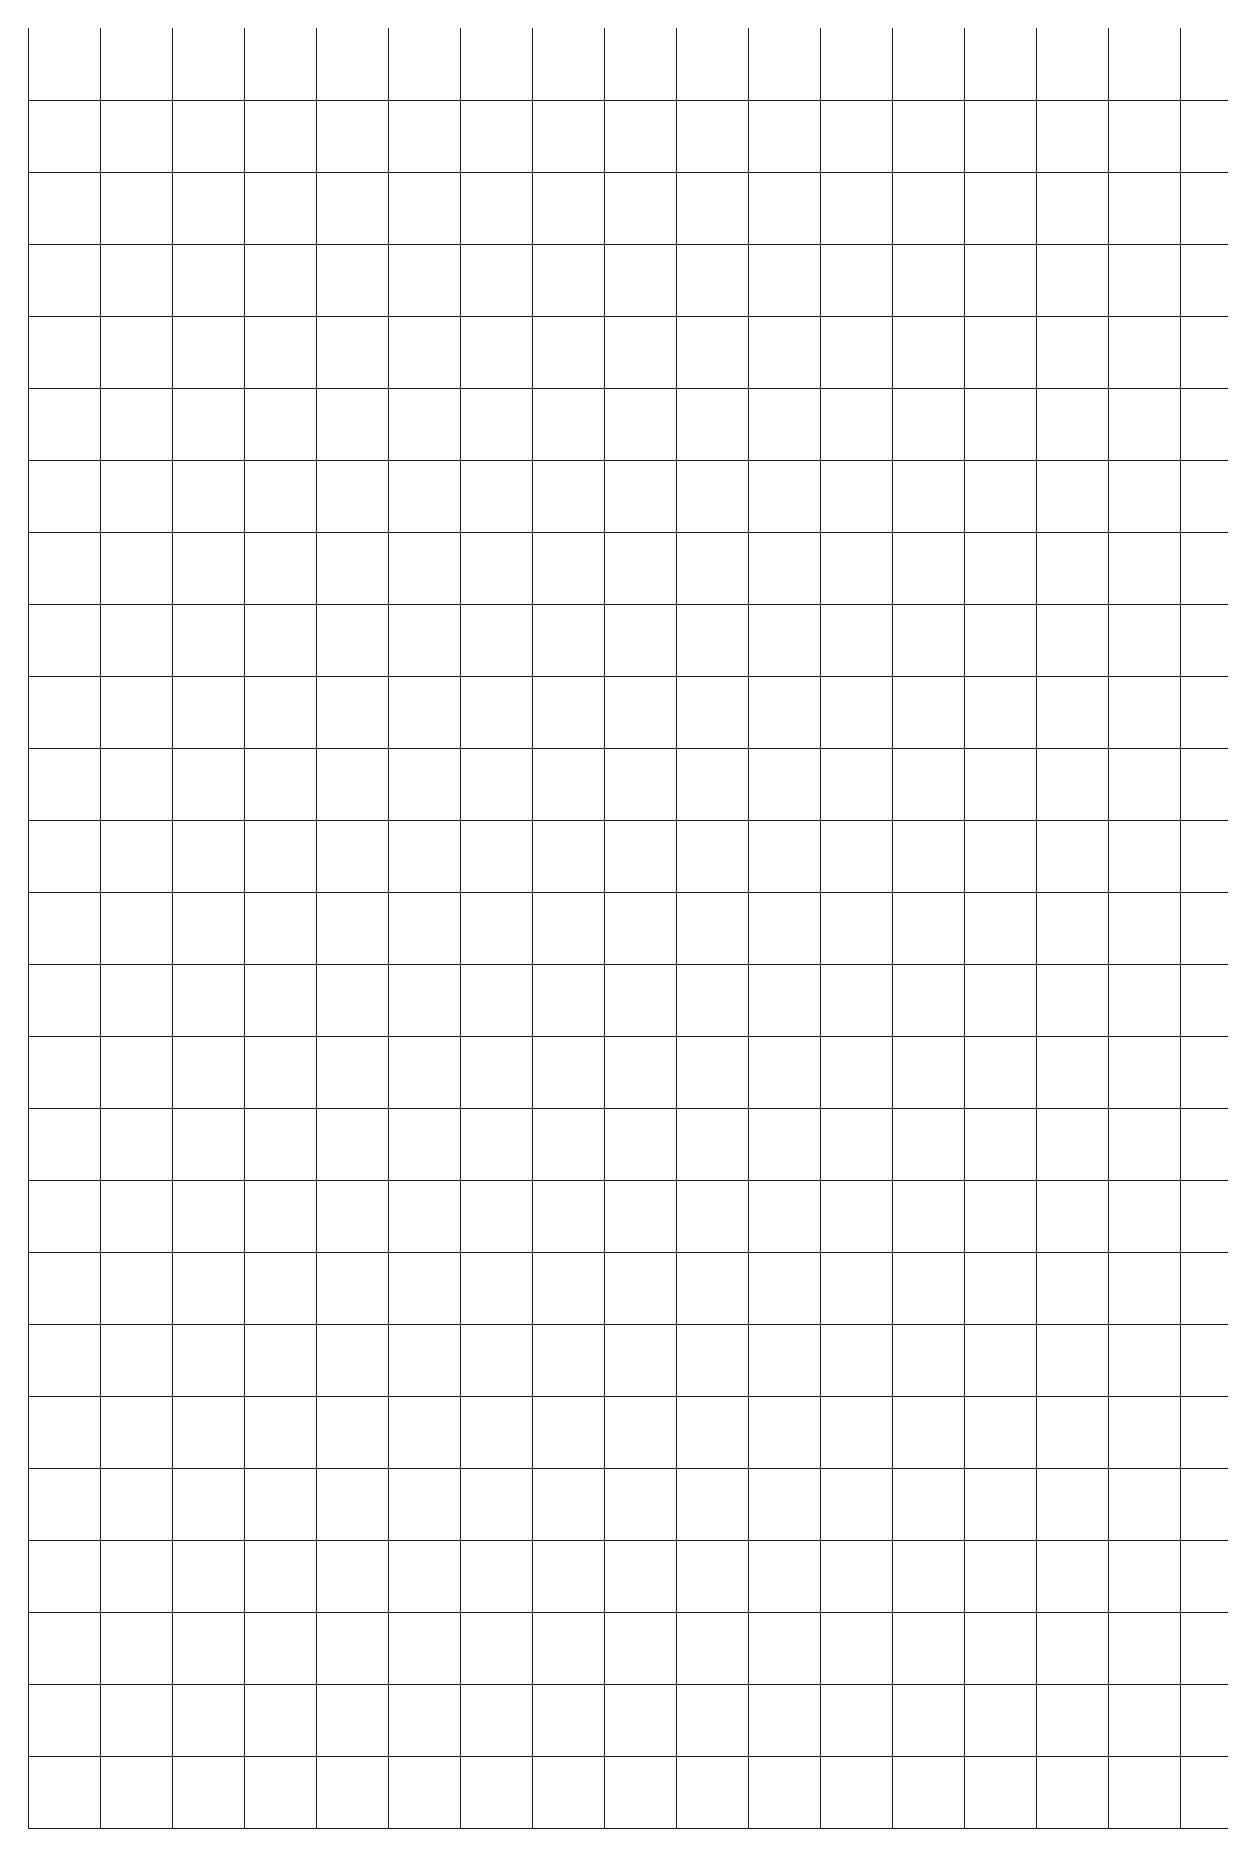
\begin{tikzpicture}[x=1in,y=1in]
        \foreach \yy in {0,0.36,...,9.0}{%
          \draw[color=gridline,line width=0.3pt] (0,\yy) -- (6,\yy);}
        \foreach \xx in {0,0.36,...,6.0}{%
          \draw[color=gridline,line width=0.3pt] (\xx,0) -- (\xx,9);}
      \end{tikzpicture}}}}

% ---- Headings -----------------------------------------------------------
\titleformat{\part}[display]
  {\normalfont\sffamily\bfseries\raggedright\color{txt}\vspace*{1.15in}\gridlayer\thispagestyle{opener}}
  {\ttfamily\fontsize{9.5}{11}\selectfont\color{accent}\MakeUppercase{Part \thepart}}
  {9pt}{\fontsize{\szTitle}{20}\selectfont\color{txt}}
  [\vspace{14pt}\textcolor{accent}{\rule{\textwidth}{1.6pt}}]
\titlespacing*{\part}{0pt}{0pt}{30pt}

\titleformat{\chapter}[display]
  {\normalfont\sffamily\bfseries\raggedright\color{txt}\gridlayer\thispagestyle{opener}}
  {\ttfamily\fontsize{9.5}{11}\selectfont\color{accent}\MakeUppercase{Chapter \thechapter}}
  {7pt}{\fontsize{\szTitle}{20}\selectfont\color{txt}}
  [\vspace{10pt}\textcolor{accent}{\rule{\textwidth}{1.6pt}}]
\titlespacing*{\chapter}{0pt}{-0.10in}{22pt}

\titleformat{\section}
  {\sffamily\bfseries\color{txt}}
  {\textcolor{accent}{\ttfamily\large\thesection}}{0.6em}{}
\titlespacing*{\section}{0pt}{16pt}{7pt}

\titleformat{\subsection}
  {\sffamily\bfseries\color{txt}}
  {\textcolor{accent}{\ttfamily\normalsize\thesubsection}}{0.55em}{}
\titlespacing*{\subsection}{0pt}{12pt}{5pt}

\titleformat{\subsubsection}
  {\sffamily\bfseries\color{txtdim}}
  {\textcolor{accentdim}{\ttfamily\small\thesubsubsection}}{0.5em}{}
\titlespacing*{\subsubsection}{0pt}{10pt}{4pt}

% ---- Contents, figures, tables -----------------------------------------
\renewcommand{\cftpartfont}{\ttfamily\bfseries\large\color{accent}}
\renewcommand{\cftchapfont}{\sffamily\bfseries\normalsize\color{txt}}
\renewcommand{\cftsecfont}{\sffamily\normalsize\color{txtdim}}
\renewcommand{\cftpartpagefont}{\ttfamily\color{txtdim}}
\renewcommand{\cftchappagefont}{\ttfamily\color{txtdim}}
\renewcommand{\cftsecpagefont}{\ttfamily\color{txtdim}}
\setcounter{tocdepth}{2}
\renewcommand{\contentsname}{Contents}
\renewcommand{\partname}{Part}
\renewcommand{\listfigurename}{Figures}
\renewcommand{\listtablename}{Tables}
\renewcommand{\figurename}{Figure}
\renewcommand{\tablename}{Table}

% ---- Running heads and folios ------------------------------------------
\renewcommand{\chaptermark}[1]{\markboth{#1}{}}
\renewcommand{\partmark}[1]{\markboth{\MakeUppercase{Part \thepart}}{}}

\pagestyle{fancy}
\fancyhf{}
\renewcommand{\headrulewidth}{0pt}
\renewcommand{\footrulewidth}{0pt}
\fancyhead[LE]{\ttfamily\fontsize{\szMeta}{9}\selectfont\color{txtdim}%
  \MakeUppercase{\bookTitle}}
\fancyhead[RO]{\ttfamily\fontsize{\szMeta}{9}\selectfont\color{txtdim}%
  \MakeUppercase{\leftmark}}
\fancyfoot[C]{\ttfamily\fontsize{\szMeta}{9}\selectfont\color{txtdim}\thepage}
\renewcommand{\headrule}{\hbox to\headwidth{%
  \color{accentdim}\leaders\hrule height 0.35pt\hfill}}
\renewcommand{\footrulewidth}{0pt}

\fancypagestyle{plain}{%
  \fancyhf{}
  \renewcommand{\headrulewidth}{0pt}
  \fancyfoot[C]{\ttfamily\fontsize{\szMeta}{9}\selectfont\color{txtdim}\thepage}}

% Chapter and part openers: folio only, no running head.
\fancypagestyle{opener}{%
  \fancyhf{}
  \renewcommand{\headrulewidth}{0pt}
  \fancyfoot[C]{\ttfamily\fontsize{\szMeta}{9}\selectfont\color{txtdim}\thepage}}

% ---- Figure and table captions -----------------------------------------
\captionsetup{font=footnotesize,labelfont={tt,bf,color=accent},
  textfont={color=txtdim},labelsep=period,width=0.96\textwidth,
  justification=justified,singlelinecheck=false,skip=7pt}
% The per-type skips are set at the start of the document: issued in the
% preamble, before the caption package knows that a table and a figure
% caption type exist, they are reported as unused.
\AtBeginDocument{%
  \captionsetup[table]{skip=6pt}%
  \captionsetup[figure]{skip=7pt}}

% ---- Epigraph (the book class does not supply one) ----------------------
\providecommand{\epigraphname}{Epigraph}
\newenvironment{epigraph}{\begin{quotation}\small\itshape}{\end{quotation}}

% ---- Cards (callout boxes) ---------------------------------------------
\newtcolorbox{takeaway}[1]{enhanced, breakable, colback=panel,
  colframe=paneledge, boxrule=0.5pt, leftrule=2.6pt, arc=0pt, outer arc=0pt,
  left=10pt, right=9pt, top=8pt, bottom=8pt,
  fonttitle=\ttfamily\bfseries\fontsize{8.2}{10}\selectfont, coltitle=accent,
  colbacktitle=panel, coltext=txt, title={#1}, before skip=12pt, after skip=12pt}
\newtcolorbox{mythbox}[1]{enhanced, breakable, colback=panel,
  colframe=paneledge, boxrule=0.5pt, leftrule=2.6pt, arc=0pt, outer arc=0pt,
  left=10pt, right=9pt, top=8pt, bottom=8pt,
  fonttitle=\ttfamily\bfseries\fontsize{8.2}{10}\selectfont, coltitle=txtdim,
  colbacktitle=panel, coltext=txt, title={#1}, before skip=12pt, after skip=12pt}
\newtcolorbox{deeper}[1]{enhanced, breakable, colback=panel,
  colframe=paneledge, boxrule=0.5pt, leftrule=1.1pt, arc=0pt, outer arc=0pt,
  left=10pt, right=9pt, top=8pt, bottom=8pt,
  fonttitle=\ttfamily\bfseries\fontsize{8.2}{10}\selectfont, coltitle=accentdim,
  colbacktitle=panel, coltext=txt, title={#1}, before skip=12pt, after skip=12pt}
\newtcolorbox{seamnote}[1]{enhanced, breakable, colback=panel,
  colframe=accent, boxrule=0.8pt, arc=0pt, outer arc=0pt,
  left=10pt, right=9pt, top=8pt, bottom=8pt,
  fonttitle=\ttfamily\bfseries\fontsize{8.2}{10}\selectfont, coltitle=accent,
  colbacktitle=panel, coltext=txt, title={#1}, before skip=12pt, after skip=12pt}

\newenvironment{keytakeaways}{%
  \begin{takeaway}{Key Takeaways}\small\begin{itemize}\setlength{\itemsep}{3pt}\setlength{\topsep}{3pt}\relax
}{%
  \end{itemize}\end{takeaway}%
}
\newenvironment{commonmyths}{%
  \begin{mythbox}{Common Myths, Straightened Out}\small\begin{itemize}\setlength{\itemsep}{3pt}\setlength{\topsep}{3pt}\relax
}{%
  \end{itemize}\end{mythbox}%
}

% ---- Math conveniences --------------------------------------------------
\newcommand{\dd}{\mathrm{d}}
\newcommand{\Tr}{\operatorname{Tr}}
\newcommand{\tr}{\operatorname{tr}}
\newcommand{\CC}{\mathbb{C}}
\newcommand{\RR}{\mathbb{R}}
\newcommand{\QQ}{\mathbb{Q}}
\newcommand{\ZZ}{\mathbb{Z}}
\newcommand{\NN}{\mathbb{N}}
\newcommand{\pp}{\partial}
\newcommand{\eps}{\varepsilon}
\newcommand{\LL}{\mathcal{L}}
\newcommand{\HH}{\mathcal{H}}
\newcommand{\OO}{\mathcal{O}}
\newcommand{\GeV}{\,\mathrm{GeV}}
\newcommand{\TeV}{\,\mathrm{TeV}}
\newcommand{\keV}{\,\mathrm{keV}}
\newcommand{\eV}{\,\mathrm{eV}}
\newcommand{\keVee}{\,\mathrm{keV}_{\mathrm{ee}}}
\newcommand{\cm}{\,\mathrm{cm}}
\newcommand{\cmtwo}{\,\mathrm{cm}^{2}}
\newcommand{\cmthree}{\,\mathrm{cm}^{3}}
\newcommand{\GeVcmthree}{\,\mathrm{GeV\,cm}^{-3}}
\newcommand{\GeVpercmsq}{\,\mathrm{GeV\,cm}^{-2}}
\newcommand{\s}{\,\mathrm{s}}
\newcommand{\kpc}{\,\mathrm{kpc}}
\newcommand{\Mpc}{\,\mathrm{Mpc}}
\newcommand{\Msun}{M_{\odot}}
\newcommand{\km}{\,\mathrm{km}}
\newcommand{\ms}{\,\mathrm{m\,s}^{-1}}
\newcommand{\kms}{\,\mathrm{km\,s}^{-1}}
\newcommand{\TW}{\,\mathrm{TW}}

% ---- Cross-reference helpers --------------------------------------------
\newcommand{\figref}[1]{Fig.~\ref{#1}}
\newcommand{\tabref}[1]{Table~\ref{#1}}

% ---- Hyperref setup -----------------------------------------------------
\hypersetup{
  pdftitle={The Shape of the Threat: Characterising Near-Earth Objects for Impact Accountability, and the Case for a Lunar Surface Array},
  pdfauthor={Gerald Enrique Nelson Mc Kenzie},
  pdfsubject={near-Earth objects, planetary defence, asteroid shape, impact energy, Torino scale, Yarkovsky drift, YORP, interferometry, lunar surface observatory, Apophis, 2024 YR4, planetary defence architecture},
  pdfkeywords={near-Earth object, NEO, planetary defence, asteroid shape, impact energy, Torino scale, Yarkovsky drift, YORP, keyhole, Apophis, 2024 YR4, interferometry, lunar surface observatory, optical ranging, parallax, shape measurement, density, rubble pile, CNEOS, impact monitoring, platform selection},
  pdfcreator={Tico Internet LLC},
  colorlinks=true,
  linkcolor=accent, citecolor=accent, urlcolor=accent,
  bookmarksnumbered=true, bookmarksopen=true
}

% ---- Index --------------------------------------------------------------
\makeindex
\newcommand{\idx}[1]{\index{#1}}
% \idxw is the same index mark, but it also PRINTS its term.  Use it
% where the mark stands in the prose for the word itself; use \idx
% where the word is already written and the mark only registers it.
% Mixing the two up is how a sentence loses its subject.
\newcommand{\idxw}[1]{\index{#1}#1}
% The index sets its page numbers in the left margin by default, which puts
% them outside the type block. Bring them inside it.
\makeatletter
\AtBeginDocument{%
  \patchcmd{\theindex}{\leftmargin\z@}{\leftmargin\@pnumwidth}{}{}}
\makeatother

% ---- Build-time generated values (page count, word count) ----------------
\IfFileExists{generated.tex}{\input{generated.tex}}{%
  \providecommand{\bookPages}{--}\providecommand{\bookWords}{--}}
